% Template for ICASSP-2021 paper; to be used with:
%          spconf.sty  - ICASSP/ICIP LaTeX style file, and
%          IEEEbib.bst - IEEE bibliography style file.
% --------------------------------------------------------------------------
\documentclass{article}
\usepackage{spconf,amsmath,graphicx}
\usepackage{hyperref}
\hypersetup{
    colorlinks=true,
    linkcolor=[rgb]{0.043,0,0.5},
    citecolor=[rgb]{0.043,0,0.5},
    urlcolor=[rgb]{0.043,0,0.5},
    filecolor=[rgb]{0.043,0,0.5},
    pdftitle={Zafar's website},
}
\usepackage{enumitem}
\usepackage[style=ieee]{biblatex}
\addbibresource{refs.bib}

% \title{Ze Adventurous French Audio Researcher (ZAFAR)}
% \title{Ze Amicable French Audio Researcher (ZAFAR)}
% \title{Ze Amusing French Audio Researcher (ZAFAR)}
% \title{Ze Annoying French Audio Researcher (ZAFAR)}
\title{Ze Awesome French Audio Researcher (ZAFAR)}

\name{Zafar Rafii}
\address{PhD in Electrical Engineering \& Computer Science}

\begin{document}

\maketitle

\begin{abstract}
We present Zafar, Ze Awesome French Audio Researcher. The proposed researcher has a PhD in electrical engineering and computer science from Northwestern University, with a focus on audio signal analysis. He has more than 40 publications, including conference papers, journal articles, and patents, with 2,400 citations in total. He is actively involved within the research community, as a reviewer, chair, and editor for several conferences and journals, an organizer of a networking meetup group in the San Francisco Bay Area, and an organizer of an international mentoring program for underrepresented groups in music information retrieval. He is currently a research scientist at Audible Magic.
\end{abstract}

\begin{keywords}
Research, audio signal analysis, separation, recognition, classification.
\end{keywords}

\section{Introduction}
\label{sec:intro}

% Patents
\nocite{patent_rafii_mar2023}
\nocite{patent_cremer_jan2023}
\nocite{patent_cremer_dec2022}
\nocite{patent_rafii_jul2022}
\nocite{patent_berrian_jun2022}
\nocite{patent_liu_jun2022}
\nocite{patent_rafii_jun2022}
\nocite{patent_rafii_mar2022}
\nocite{patent_rafii_oct2021}
\nocite{patent_rafii_may2021}
\nocite{patent_rafii_oct2020}
\nocite{patent_rafii_jul2020}
\nocite{patent_coover_mar2020}
\nocite{patent_pardo_jul2015}

% Journal Articles
\nocite{article_rafii_nov2024}
\nocite{article_rafii_may2022}
\nocite{article_rafii_nov2018}
\nocite{article_rafii_aug2018}
\nocite{article_rafii_dec2014}
\nocite{article_liutkus_aug2014}
\nocite{article_rafii_jan2013}
\nocite{article_sabin_jun2013}

% Conference Proceedings
\nocite{inproceedings_vartakavi_aug2021}
\nocite{inproceedings_kim_sep2018}
\nocite{inproceedings_seetharaman_mar2017}
\nocite{inproceedings_fitzgerald_mar2017}
\nocite{inproceedings_liutkus_feb2017}
\nocite{inproceedings_ono_aug2015}
\nocite{inproceedings_rafii_apr2015}
\nocite{inproceedings_liutkus_apr2015}
\nocite{inproceedings_fitzgerald_jun2014}
\nocite{inproceedings_liutkus_may2014}
\nocite{inproceedings_rafii_may2014}
\nocite{inproceedings_rafii_nov2013}
\nocite{inproceedings_rafii_may2013}
\nocite{inproceedings_rafii_oct2012}
\nocite{inproceedings_liutkus_mar2012}
\nocite{inproceedings_cartwright_aug2011}
\nocite{inproceedings_rafii_may2011}
\nocite{inproceedings_rafii_may2011_2}
\nocite{inproceedings_rafii_oct2009}

% Chapter Books
\nocite{inbook_pardo_2018}
\nocite{inbook_rafii_2014}

% Technical Reports
\nocite{report_rafii_2009}

% Tutorials
\nocite{misc_mcdermott_oct2012}

% Workshops
\nocite{misc_rafii_jun2014}
\nocite{misc_rafii_jun2011}
\nocite{misc_rafii_dec2007}

% Talks
\nocite{misc_rafii_mar2021}
\nocite{misc_rafii_apr2018}
\nocite{misc_rafii_july2015}
\nocite{misc_rafii_may2015}
\nocite{misc_rafii_jul2011}

% Lectures
\nocite{misc_rafii_dec2014_4}
\nocite{misc_rafii_dec2014_3}
\nocite{misc_rafii_dec2014_2}
\nocite{misc_rafii_dec2014}

% Data Sets
\nocite{online_rafii_2019}
\nocite{online_rafii_2017}


The proposed researcher is named Zafar Rafii. He received a PhD in electrical engineering and computer science from \href{https://www.northwestern.edu/}{Northwestern University} in 2014. He was with the \href{https://interactiveaudiolab.github.io/}{Interactive Audio Lab} under the supervision of professor \href{https://bryan-pardo.github.io/}{Bryan Pardo}. Prior to that, he was a research engineer at \href{https://audionamix.com/}{Audionamix}, in France. He was then a research engineer manager at \href{https://www.gracenote.com/}{Gracenote}. He is now a research scientist at \href{https://www.audiblemagic.com/}{Audible Magic}.

\begin{figure}[!htb]
\centering
% 
\includegraphics[width=0.5\columnwidth]{Images/adventurous.png}
% 
\includegraphics[width=0.5\columnwidth]{Images/amicable.png}
% 
\includegraphics[width=0.5\columnwidth]{Images/amusing.png}
% 
\includegraphics[width=0.5\columnwidth]{Images/annoying.png}

\includegraphics[width=0.5\columnwidth]{Images/awesome.png}
\caption{Overview of the proposed researcher.}
\label{fig:zafar}
\end{figure}

The proposed researcher has interest and expertise in audio signal analysis. He has worked on a number of projects, including:
\begin{itemize}[noitemsep,topsep=0pt]
\item Blind source separation
\item Spatial source separation
\item Digital audio effects
\item Audio fingerprinting
\item Cover song identification
\item Audio encoding analysis
\item Audio beamforming
\item Audio watermarking
\item Audio/video segmentation
\item Audio classification
\end{itemize}

For more information on the proposed researcher, the reader is referred to the following materials:
\begin{itemize}[noitemsep,topsep=0pt]
\item \href{http://zafarrafii.com/Zafar Rafii - CV.pdf}{CV}
\item \href{https://github.com/zafarrafii}{GitHub}
\item \href{https://www.linkedin.com/in/zafarrafii/}{LinkedIn}
\item \href{https://scholar.google.com/citations?user=8wbS2EsAAAAJ&hl=en}{Google Scholar}
\end{itemize}

For other relevant information related to the proposed researcher, such as the meetups he organizes, the mentoring program he is involved in, or the audio dataset he created, the reader is referred to the following links:
\begin{itemize}[noitemsep,topsep=0pt]
\item \href{https://www.meetup.com/bishbash/}{SF-BISH Bash meetup}
\item \href{https://wimir.wordpress.com/}{Widening Inclusion in Music Information Retrieval}
\item \href{https://sigsep.github.io/datasets/musdb.html#musdb18-compressed-stems}{MUSDB18 dataset}
\end{itemize}

The rest of the website is organized as follows. In \hyperref[sec:research]{Section 2}, we present a selection of projects in which the proposed researcher has worked. In \hyperref[sec:repet]{Section 3}, we introduce his PhD thesis work on the REpeating Pattern Extraction Technique (REPET) for blind source separation. In \hyperref[sec:codes]{Section 4}, we share links to his GitHub repositories where some of his source codes reside. In \hyperref[sec:refs]{Section 5}, we provide references to all of his publications, presentations, and other materials.


\section{Research}
\label{sec:research}

\subsection{Adaptive Reverberation Tool (2008)}
\label{ssec:reverb}

People often think about sound in terms of subjective concepts which do not necessarily have known mappings onto the controls of existing audio tools. For example, a bass player may wish to use a reverberation effect to make her/his bass sound more "boomy", but unfortunately there is no "boomy" knob to be found. We developed a system that can quickly learn an audio concept from a user (e.g., a "boomy" effect) and generate a simple controller than can manipulate sounds in terms of that audio concept (e.g., make a sound more "boomy"), bypassing the bottleneck of technical knowledge of complex interfaces and individual differences in subjective terms.

For this study, we focused on reverberation effects. We developed a digital reverberator, mapping the parameters of the digital filters to measures of the reverberation effect, so that the reverberator can be controlled through meaningful descriptors such as "reverberation time" or "spectral centroid." In the learning process, a sound is first modified by a series of reverberation settings using the reverberator. The user then listens and rates each modified sound as to how well it fits the audio concept she/he has in mind. The ratings are finally mapped onto the controls of the reverberator and a simple controller is built with which the user is able to manipulate the degree of her/his audio concept on a sound. Several experiments conducted on human subjects showed that the system learns quickly (under 3 minutes), predicts user responses well (mean correlation of 0.75), and meets users' expectations (average human rating of 7.4 out of 10).

\begin{figure}[!htb]
\centering
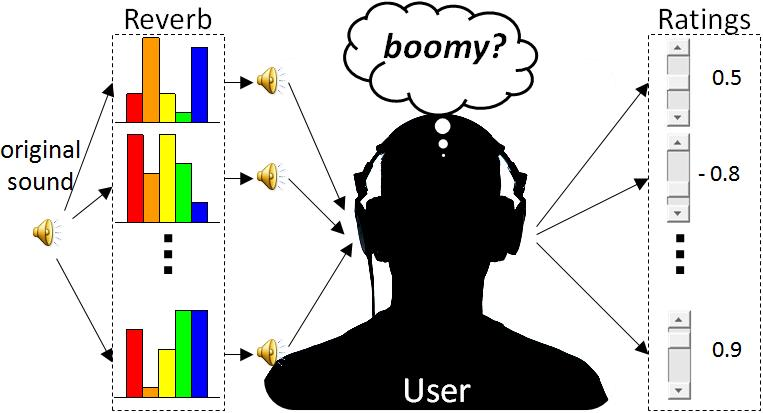
\includegraphics[width=\columnwidth]{Images/reverberation.jpg}
\caption{A listener rating a sound modified by a series of reverberation settings as to how well it fits the audio concept of "boomy" they have in mind.}
\label{fig:reverb}
\end{figure}

For more information on this project, the reader is referred to \cite{article_sabin_jun2013}, \cite{inproceedings_rafii_oct2009}, and 
\cite{report_rafii_2009}.


\subsection{DUET using the CQT (2011)}
\label{ssec:duet}

The Degenerate Unmixing Estimation Technique (DUET) is a blind source separation method that can separate an arbitrary number of unknown sources using a single stereo mixture. DUET builds a two-dimensional histogram from the amplitude ratio and phase difference between channels, where each peak indicates a source, with peak location corresponding to the mixing parameters associated with that source. Provided that the time-frequency bins of the sources do not overlap too much - an assumption generally validated by speech mixtures, DUET partitions the time-frequency representation of the mixture by assigning each bin to the source with the closest mixing parameters. However, when time-frequency bins of the sources start to overlap more - as generally seen in music mixtures when using the common short-time Fourier transform (STFT), peaks start to fuse in the 2d histogram and DUET cannot perform separation effectively.

\begin{figure}[!htb]
\centering
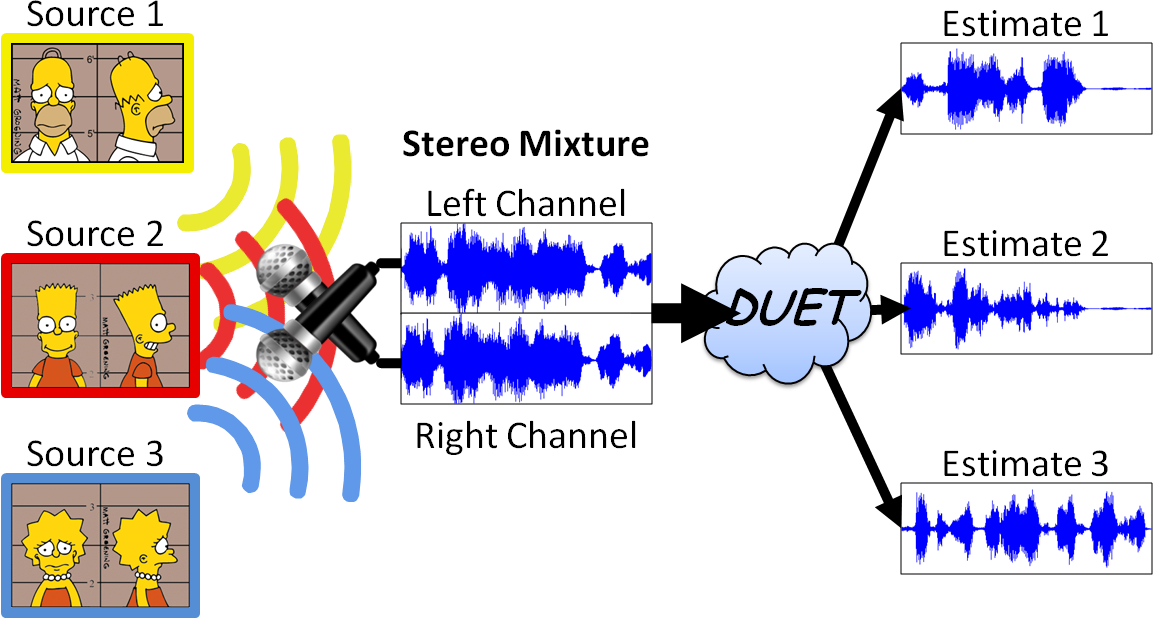
\includegraphics[width=\columnwidth]{Images/duet.png}
\caption{Blind source separation of a stereo recording of Homer, Bart, and Lisa using DUET.}
\label{fig:duet}
\end{figure}

We proposed to improve peak/source separation in DUET by building the 2d histogram from an alternative time-frequency representation based on the constant-Q transform (CQT). Unlike the Fourier transform, the CQT has a logarithmic frequency resolution, mirroring the human auditory system and matching the geometrically spaced frequencies of the Western music scale, therefore better adapted to music mixtures. We also proposed other contributions to enhance DUET, such as adaptive boundaries for the 2d histogram to improve peak resolving when sources are spatially too close to each other, and Wiener filtering to improve source reconstruction. Experiments on mixtures of piano notes and harmonic sources showed that peak/source separation is overall improved, especially at low octaves (under 200 Hz) and for small mixing angles (under ${\pi}/{6}$ rad).

Unlike the classic DUET based on the Fourier transform, DUET combined with the CQT can resolve adjacent pitches in low octaves as well as in high octaves thanks to the log frequency resolution of the CQT:
\begin{itemize}[noitemsep,topsep=0pt]
\item \href{Audio/DUET/piano_mixture.mp3}{Mixture of 3 piano notes}
\item Estimates: \href{Audio/DUET/A2_estimated.mp3}{A2} - \href{Audio/DUET/Bb2_estimated.mp3}{Bb2} -  \href{Audio/DUET/B2_estimated.mp3}{B2}
\item Originals: \href{Audio/DUET/A2_original.mp3}{A2} - \href{Audio/DUET/Bb2_original.mp3}{Bb2} - \href{Audio/DUET/B2_original.mp3}{B2}
\end{itemize}

DUET combined with the CQT and adaptive boundaries helps to improve separation when sources have low pitches (for example, here, between the two cellos) and/or are spatially too close to each other:
\begin{itemize}[noitemsep,topsep=0pt]
\item \href{Audio/DUET/instruments_mixture.mp3}{Mixture of 4 instruments}
\item Estimates: \href{Audio/DUET/cello1_estimated.mp3}{cello 1} - \href{Audio/DUET/cello2_estimated.mp3}{cello 2} - \href{Audio/DUET/flute_estimated.mp3}{flute} - \href{Audio/DUET/strings_estimated.mp3}{strings}
\item Originals: \href{Audio/DUET/cello1_original.mp3}{cello 1} - \href{Audio/DUET/cello2_original.mp3}{cello 2} - \href{Audio/DUET/flute_original.mp3}{flute} - \href{Audio/DUET/strings_original.mp3}{strings}
\end{itemize}

For more information on this project, the reader is referred to \cite{inproceedings_rafii_may2011_2}.


\subsection{Live Music Fingerprinting (2014)}
\label{ssec:live} 

Suppose that you are at a music festival checking on an artist, and you would like to quickly know about the song that is being played (e.g., title, lyrics, album, etc.). If you have a smartphone, you could record a sample of the live performance and compare it against a database of existing recordings from the artist. Services such as Shazam or SoundHound will not work here, as this is not the typical framework for audio fingerprinting or query-by-humming systems, as a live performance is neither identical to its studio version (e.g., variations in instrumentation, key, tempo, etc.) nor it is a hummed or sung melody. We propose an audio fingerprinting system that can deal with live version identification by using image processing techniques. Compact fingerprints are derived using a log-frequency spectrogram and an adaptive thresholding method, and template matching is performed using the Hamming similarity and the Hough Transform.

\begin{figure}[!htb]
\centering
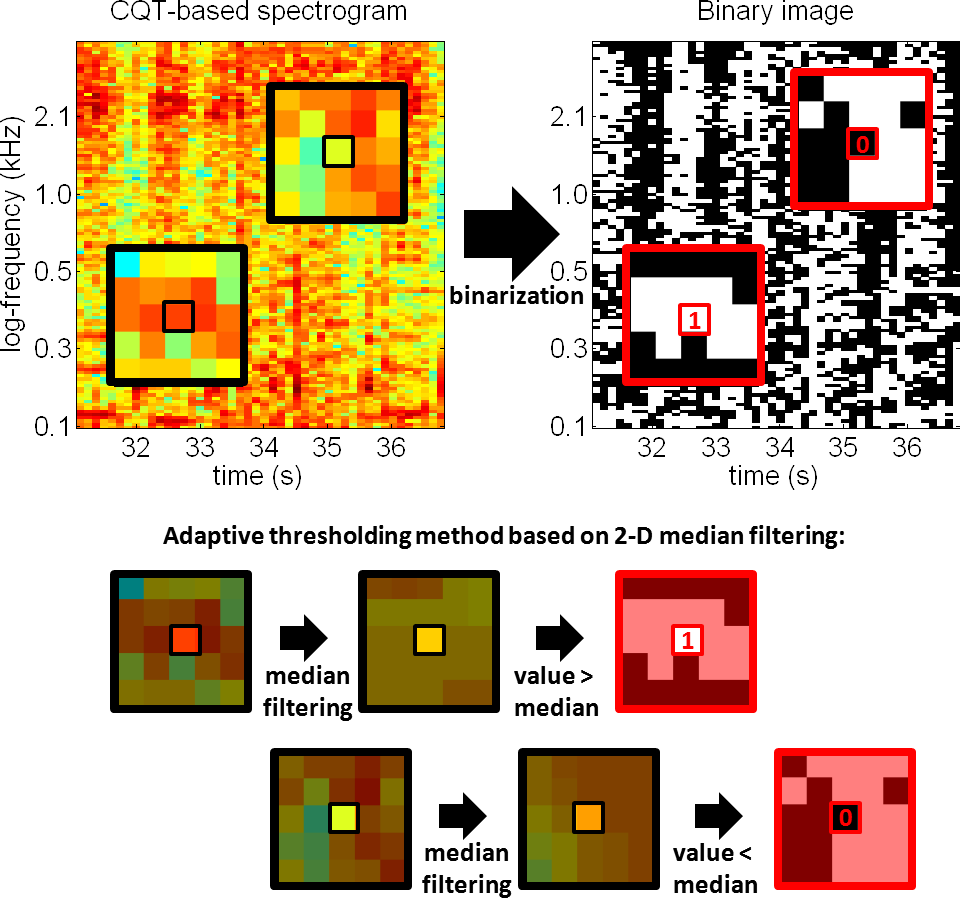
\includegraphics[width=\columnwidth]{Images/thresholding.png}
\caption{Overview of the fingerprinting stage. The audio signal is first transformed into a log-frequency spectrogram by using the CQT. The CQT-based spectrogram is then transformed into a binary image by using an adaptive thresholding method.}
\label{fig:thresholding}
\end{figure}

For more information on this project, the reader is referred to \cite{inproceedings_rafii_may2014}.


\subsection{Lossy Audio Compression Identification (2018)}
\label{ssec:compression}

We propose a system which can estimate from an audio recording that has previously undergone lossy compression the parameters used for the encoding, and therefore identify the corresponding lossy coding format. The system analyzes the audio signal and searches for the compression parameters and framing conditions which match those used for the encoding. In particular, we propose a new metric for measuring traces of compression which is robust to variations in the audio content and a new method for combining the estimates from multiple audio blocks which can refine the results. We evaluated this system with audio excerpts from songs and movies, compressed into various coding formats, using different bit rates, and captured digitally as well as through analog transfer. Results showed that our system can identify the correct format in almost all cases, even at high bitrates and with distorted audio, with an overall accuracy of 0.96.

\begin{figure}[!htb]
\centering
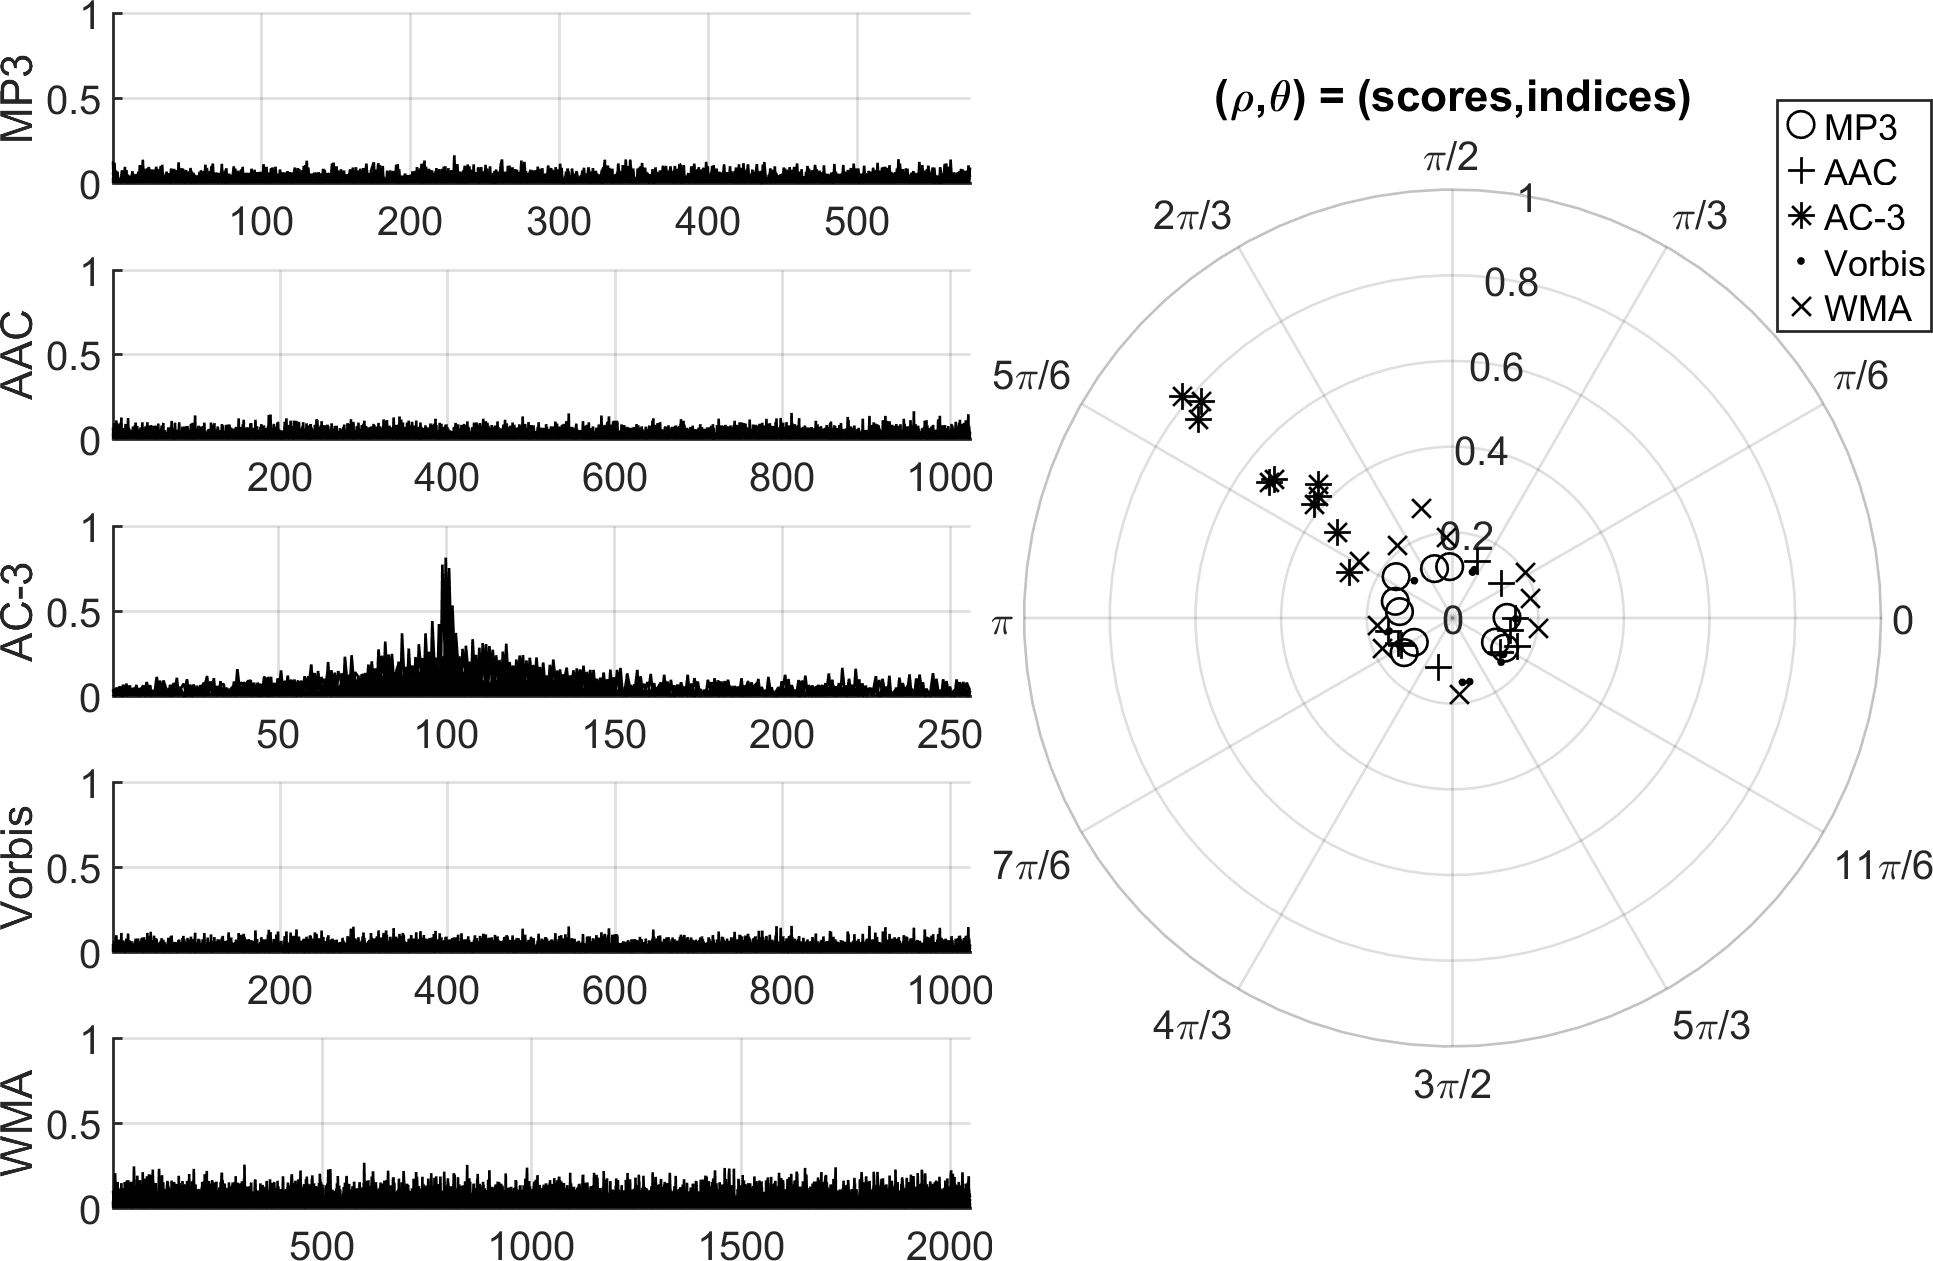
\includegraphics[width=\columnwidth]{Images/compression.png}
\caption{Results for an audio example encoded with AC-3. The system identified traces of compression corresponding to AC-3, but not to other lossy coding formats such as MP3, AAC, Vorbis, or WMA.}
\label{fig:compression}
\end{figure}

For more information on this project, the reader is referred to \cite{inproceedings_kim_sep2018}.


\subsection{Sliding DFT with Kernel Windowing (2018)}
\label{ssec:sdft}

The sliding discrete Fourier transform (SDFT) is an efficient method for computing the N-point DFT of a given signal starting at a given sample from the N-point DFT of the same signal starting at the previous sample. However, the SDFT does not allow the use of a window function, generally incorporated in the computation of the DFT to reduce spectral leakage, as it would break its sliding property. We show how windowing can be included in the SDFT by using a kernel derived from the window function, while keeping the process computationally efficient. In addition, this approach allows for turning other transforms, such as the modified discrete cosine transform (MDCT), into efficient sliding versions of themselves.

\begin{figure}[!htb]
\centering
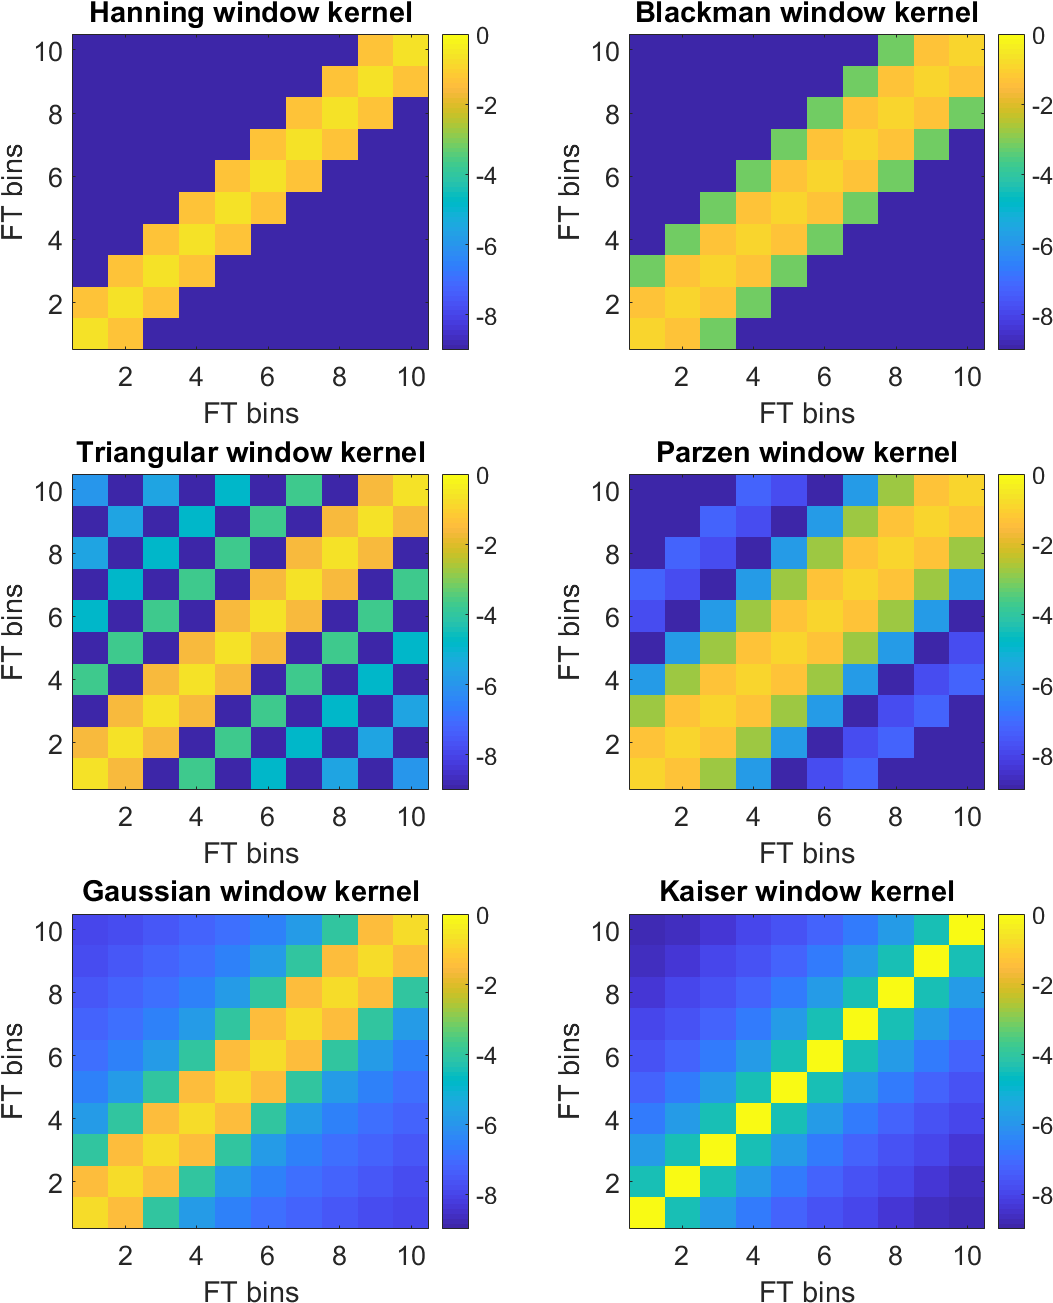
\includegraphics[width=\columnwidth]{Images/kernels.png}
\caption{Kernels derived from the Hanning, Blackman, triangular, Parzen, Gaussian (with $\alpha$ = 2.5), and Kaiser (with $\beta$ = 0.5) windows. The kernels were derived for an N-point DFT where N = 2,048 samples. Only the first 100 coefficients at the bottom-left corner of the N-by-N kernels are shown. The values are displayed in log of amplitude.}
\label{fig:kernels}
\end{figure}

For more information on this project, the reader is referred to \cite{article_rafii_nov2018}.


\subsection{Constant-Q Harmonic Coefficients (2022)}
\label{ssec:cqhc}

Timbre is the attribute of sound that makes, for example, two musical instruments playing the same note sound different. It is typically associated with the spectral (but also the temporal) envelope and assumed to be independent from the pitch (but also the loudness) of the sound. We show how to design a simple but effective pitch-independent timbre feature, well adapted to musical data, by deriving it from the constant-Q transform (CQT), a log-frequency transform that matches the typical Western musical scale. The decomposition of the CQT spectrum into an energy-normalized pitch component and a pitch-normalized spectral component is demonstrated, the latter from which a number of harmonic coefficients are extracted. The discriminative powers of these constant-Q harmonic coefficients (CQHCs) are then evaluated on the NSynth data set, a publicly available, large-scale data set of musical notes, where they are compared with the mel-frequency cepstral coefficients (MFCCs), a feature originally designed for speech recognition but commonly used to characterize timbre in music.

\begin{figure}[!htb]
	\centering
	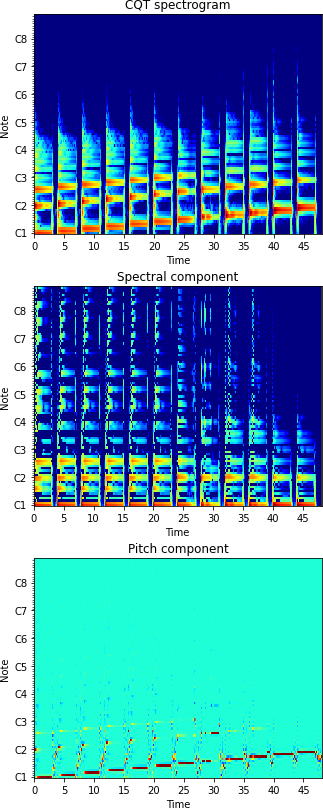
\includegraphics[width=0.6\columnwidth]{Images/cqtdeconv.png}
	\caption{The deconvolution of the CQT spectrogram (shown in dB) of 12 acoustic bass notes playing from C1 to B1, into a pitch-normalized spectral component (shown in dB), and an energy-normalized pitch component (shown in [0, 1]).}
	\label{fig:cqtdeconv}
\end{figure}

An online Python implementation of CQHCs is provided with some examples \href{https://github.com/zafarrafii/CQHC-Python}{here}. For more information on this project, the reader is referred to \cite{article_rafii_may2022}.


\subsection{Cheap Music Detection using a Simple Multilayer Perceptron with Temporal Integration (2024)}
\label{ssec:music_detection}

We will show how to design a cheap system for detecting when music is present in audio recordings. We will make use of a small neural network consisting of a simple multilayer perceptron (MLP), along with compact features derived from the mel spectrogram by means of temporal integration. Temporal integration is the process of combining information over time, for example, by computing statistics over a sequence of spectra in audio. We will experiment with common statistics and compare the performances of various small MLPs, with each other and with more complex models, on two large music detection datasets. We note that this article does not claim to propose a state-of-the-art music detection model but rather to demonstrate how anybody can design their own efficient system from scratch using simple ideas and with limited resources.

\begin{figure}[!htb]
	\centering
	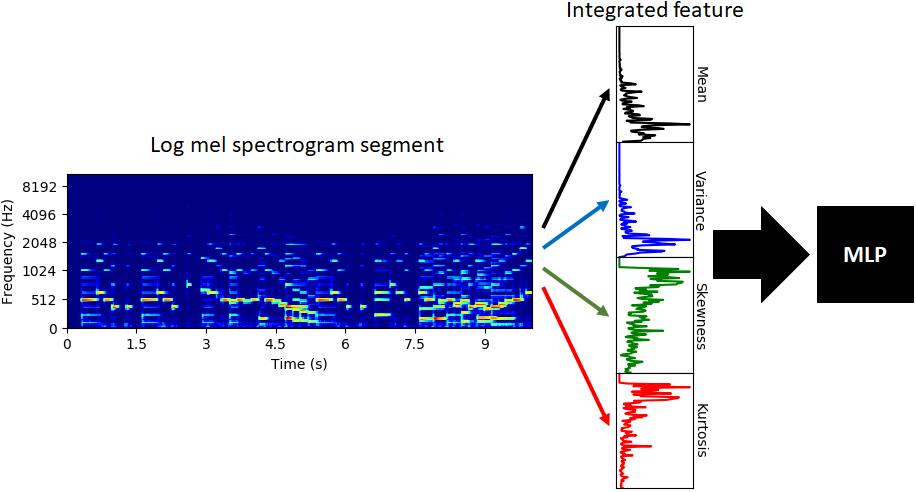
\includegraphics[width=1.0\columnwidth]{Images/temporal_integration.png}
	\caption{The temporal integration over a 10-s segment of a log mel spectrogram by computing the first four moments (mean, variance, skewness, and
kurtosis) and concatenating them into a 1D feature that can then be fed into an MLP..}
	\label{fig:temporal_integration}
\end{figure}

For more information on this project, the reader is referred to \cite{article_rafii_nov2024}.


\section{REPET}
\label{sec:repet}

Repetition is a fundamental element in generating and perceiving structure. In audio, mixtures are often composed of structures where a repeating background signal is superimposed with a varying foreground signal. On this basis, we present the REpeating Pattern Extraction Technique (REPET), a simple approach for separating the repeating background from the non-repeating foreground in an audio mixture. The basic idea is to find the repeating elements in the mixture, derive the underlying repeating models, and extract the repeating background by comparing the models to the mixture. Unlike other separation approaches, REPET does not depend on special parameterizations, does not rely on complex frameworks, and does not require external information. Because it is only based on repetition, it has the advantage of being simple, fast, blind, and therefore completely and easily automatable.

\begin{figure}[!htb]
\centering
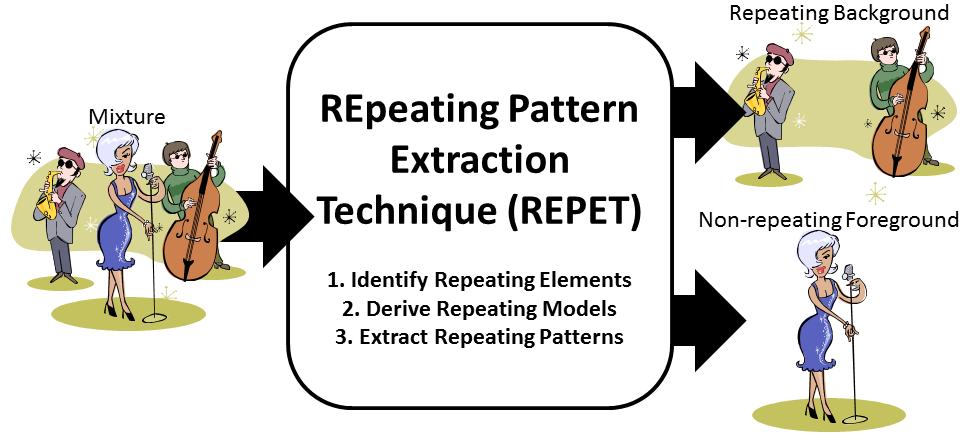
\includegraphics[width=\columnwidth]{Images/repet.png}
\caption{Overview of REPET.}
\label{fig:repet}
\end{figure}

\subsection{Original REPET (2011)}
\label{ssec:repet_original}

The original REPET aims at identifying and extracting the repeating patterns in an audio mixture, by estimating a period of the underlying repeating structure and modeling a segment of the periodically repeating background.

\begin{figure}[!htb]
\centering
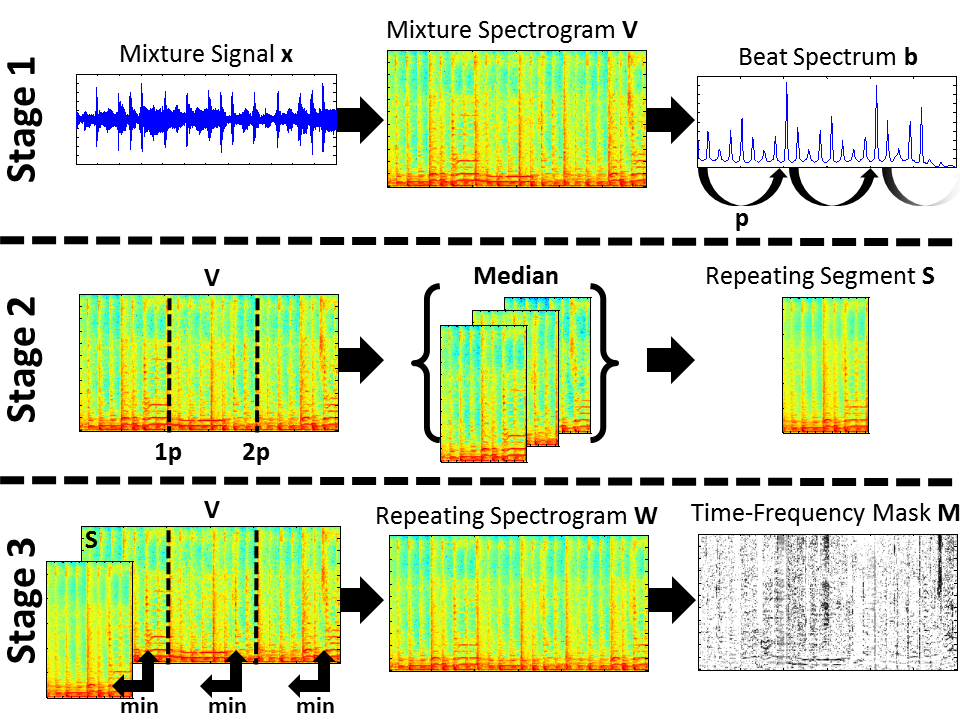
\includegraphics[width=\columnwidth]{Images/repet_original_overview.png}
\caption{Overview of the original REPET. Stage 1: calculation of the beat spectrum b and estimation of a repeating period p. Stage 2: segmentation of the mixture spectrogram V and calculation of the repeating segment S. Stage 3: calculation of the repeating spectrogram W and derivation of the time-frequency mask M.}
\label{fig:repet_original_overview}
\end{figure}

Experiments on a data set of song clips showed that REPET can be effectively applied for music/voice separation. Experiments also showed that REPET can be combined with other methods to improve background/foreground separation; for example, it can be used as a preprocessor to pitch detection algorithms to improve melody extraction, or as a postprocessor to a singing voice separation algorithm to improve music/voice separation.

\begin{figure}[!htb]
\centering
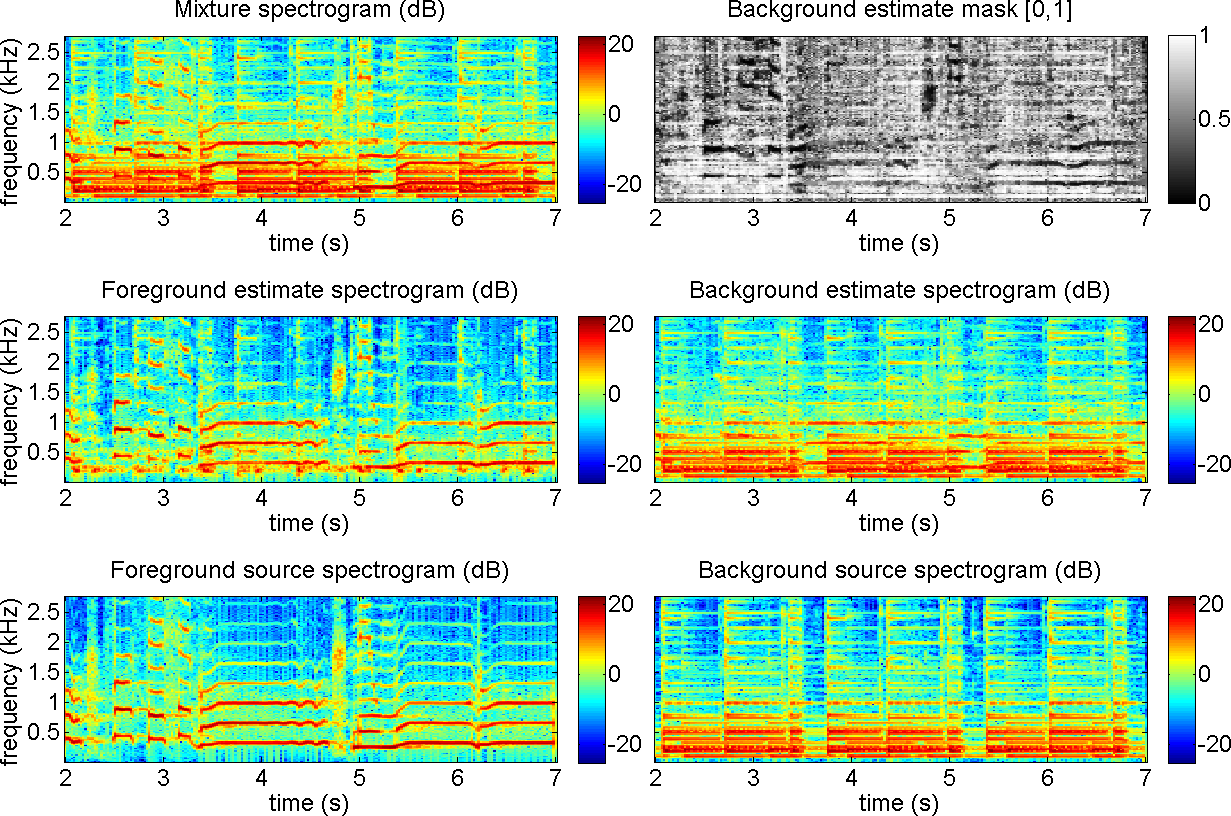
\includegraphics[width=\columnwidth]{Images/repet_original_example.png}
\caption{Music/voice separation using REPET. The mixture is a female singer (foreground) singing over a guitar accompaniment (background). The guitar has a repeating chord progression that is stable along the song. The spectrograms and the mask are shown for 5 seconds and up to 2.5 kHz.}
\label{fig:repet_original_example}
\end{figure}

\begin{itemize}[noitemsep,topsep=0pt]
\item \href{Audio/REPET/dev1__tamy-que_pena_tanto_faz__snip_6_19__mix.wav}{Mixture}
\item Estimates: \href{Audio/REPET/dev1__tamy-que_pena_tanto_faz__snip_6_19__mix_background.wav}{background} - \href{Audio/REPET/dev1__tamy-que_pena_tanto_faz__snip_6_19__mix_foreground.wav}{foreground}
\item Originals: \href{Audio/REPET/dev1__tamy-que_pena_tanto_faz__snip_6_19__guitar.wav}{accompaniment} - \href{Audio/REPET/dev1__tamy-que_pena_tanto_faz__snip_6_19__vocals.wav}{vocals}
\end{itemize}

REPET can be easily extended to handle varying repeating structures, by simply applying the method along time, on individual segments or via a sliding window. Experiments on a data set of full-track real-world songs showed that this method can be effectively applied for music/voice separation.

For more information on this project, the reader is referred to \cite{inproceedings_rafii_may2011}, \cite{article_rafii_jan2013}, and \cite{inbook_rafii_2014}.


\subsection{Adaptive REPET (2012)}
\label{ssec:repet_adaptive}

The original REPET works well when the repeating background is relatively stable (e.g., a verse or the chorus in a song); however, the repeating background can also vary over time (e.g., a verse followed by the chorus in the song). The adaptive REPET is an extension of the original REPET that can handle varying repeating structures, by estimating the time-varying repeating periods and extracting the repeating background locally, without the need for segmentation or windowing.

\begin{figure}[!htb]
\centering
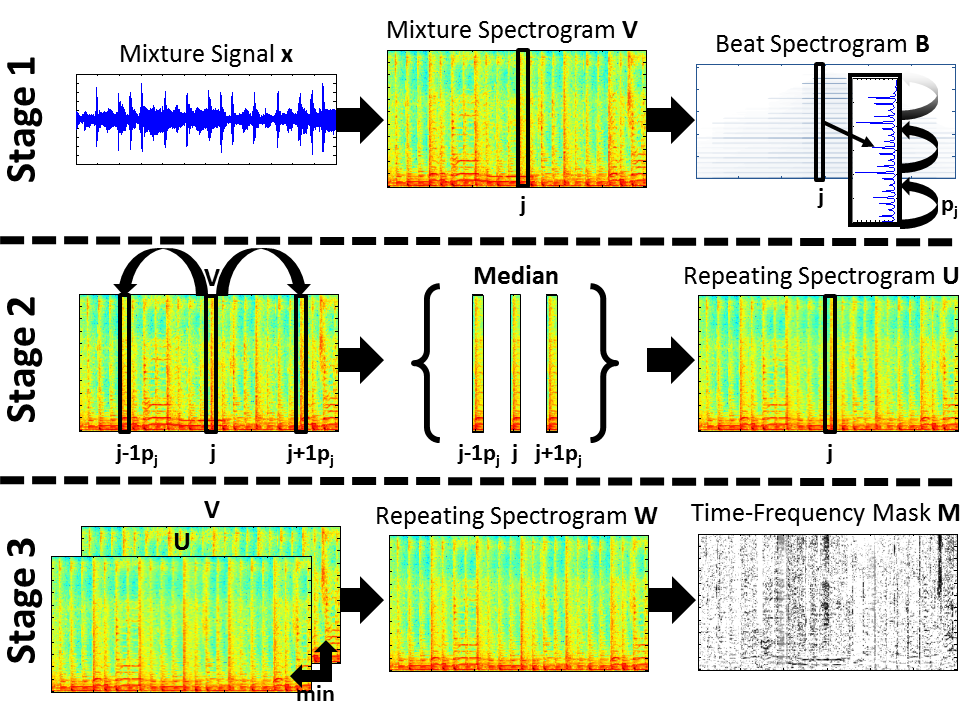
\includegraphics[width=\columnwidth]{Images/repet_adaptive_overview.png}
\caption{Overview of the adaptive REPET. Stage 1: calculation of the beat spectrogram B and estimation of the repeating periods pj’s. Stage 2: filtering of the mixture spectrogram V and calculation of an initial repeating spectrogram U. Stage 3: calculation of the refined repeating spectrogram W and derivation of the time-frequency mask M.}
\label{fig:repet_adaptive_overview}
\end{figure}

Experiments on a data set of full-track real-world songs showed that the adaptive REPET can be effectively applied for music/voice separation.

\begin{figure}[!htb]
\centering
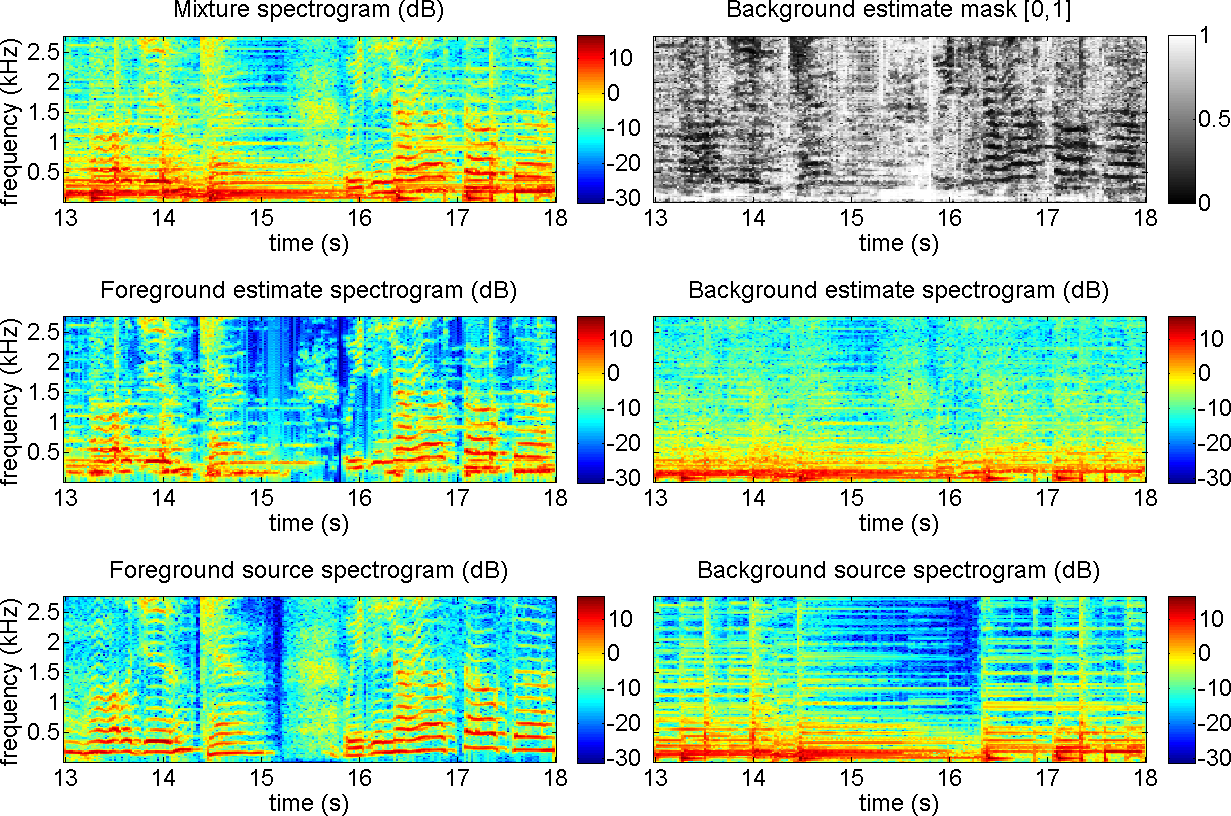
\includegraphics[width=\columnwidth]{Images/repet_adaptive_example.png}
\caption{Music/voice separation using the adaptive REPET. The mixture is a male singer (foreground) singing over a guitar and drums accompaniment (background). The guitar has a repeating chord progression that changes around 15 seconds. The spectrograms and the mask are shown for 5 seconds and up to 2.5 kHz.}
\label{fig:repet_adaptive_example}
\end{figure}

\begin{itemize}[noitemsep,topsep=0pt]
\item \href{Audio/REPET/dev2__another_dreamer-the_ones_we_love__snip_69_94__mix.wav}{Mixture}
\item Estimates: \href{Audio/REPET/dev2__another_dreamer-the_ones_we_love__snip_69_94__mix_background.wav}{background} - \href{Audio/REPET/dev2__another_dreamer-the_ones_we_love__snip_69_94__mix_foreground.wav}{foreground}
\item Originals: \href{Audio/REPET/dev2__another_dreamer-the_ones_we_love__snip_69_94__mix-vocals.wav}{accompaniment} - \href{Audio/REPET/dev2__another_dreamer-the_ones_we_love__snip_69_94__vocals.wav}{vocals}
\end{itemize}

For more information on this project, the reader is referred to \cite{inproceedings_liutkus_mar2012} and \cite{inbook_rafii_2014}.


\subsection{REPET-SIM (2012)}
\label{ssec:repet_sim}

The REPET methods work well when the repeating background has periodically repeating patterns (e.g., jackhammer noise); however, the repeating patterns can also happen intermittently or without a global or local periodicity (e.g., frogs by a pond). REPET-SIM is a generalization of REPET that can also handle non-periodically repeating structures, by using a similarity matrix to identify the repeating elements.

\begin{figure}[!htb]
\centering
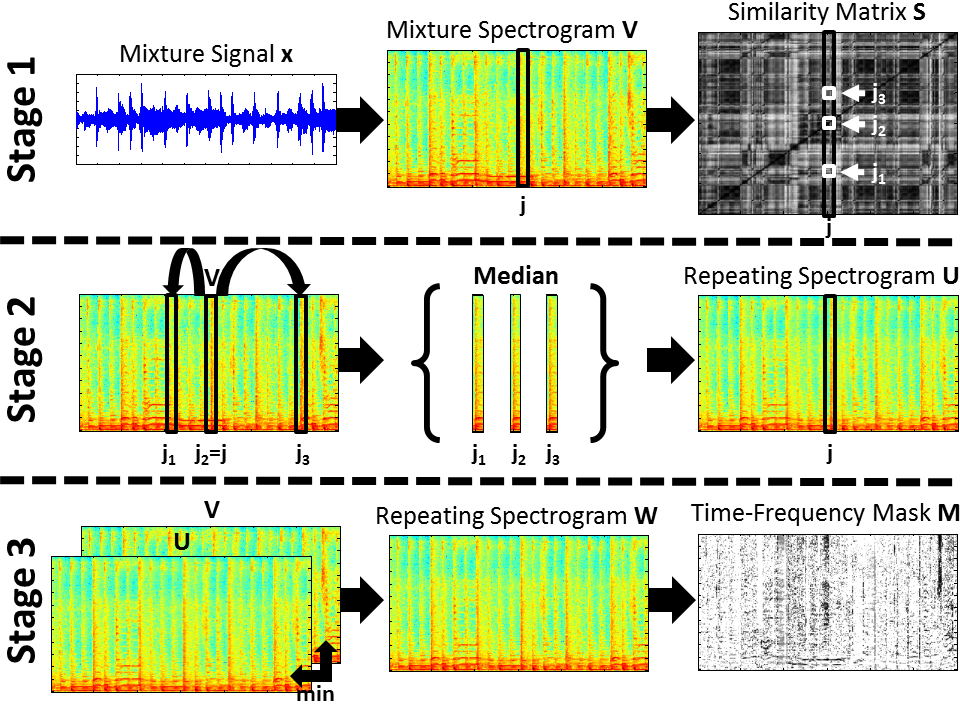
\includegraphics[width=\columnwidth]{Images/repet_sim_overview.png}
\caption{Overview of REPET-SIM. Stage 1: calculation of the similarity matrix S and estimation of the repeating indices jk’s. Stage 2: filtering of the mixture spectrogram V and calculation of an initial repeating spectrogram U. Stage 3: calculation of the refined repeating spectrogram W and derivation of the time-frequency mask M.}
\label{fig:repet_sim_overview}
\end{figure}

Experiments on a data set of full-track real-world songs showed that REPET-SIM can be effectively applied for music/voice separation.

REPET-SIM can be easily implemented online to handle real-time computing, particularly for real-time speech enhancement. The online REPET-SIM simply processes the time frames of the mixture one after the other given a buffer that temporally stores past frames. Experiments on a data set of two-channel mixtures of one speech source and real-world background noise showed that the online REPET-SIM can be effectively applied for real-time speech enhancement.

\begin{figure}[!htb]
\centering
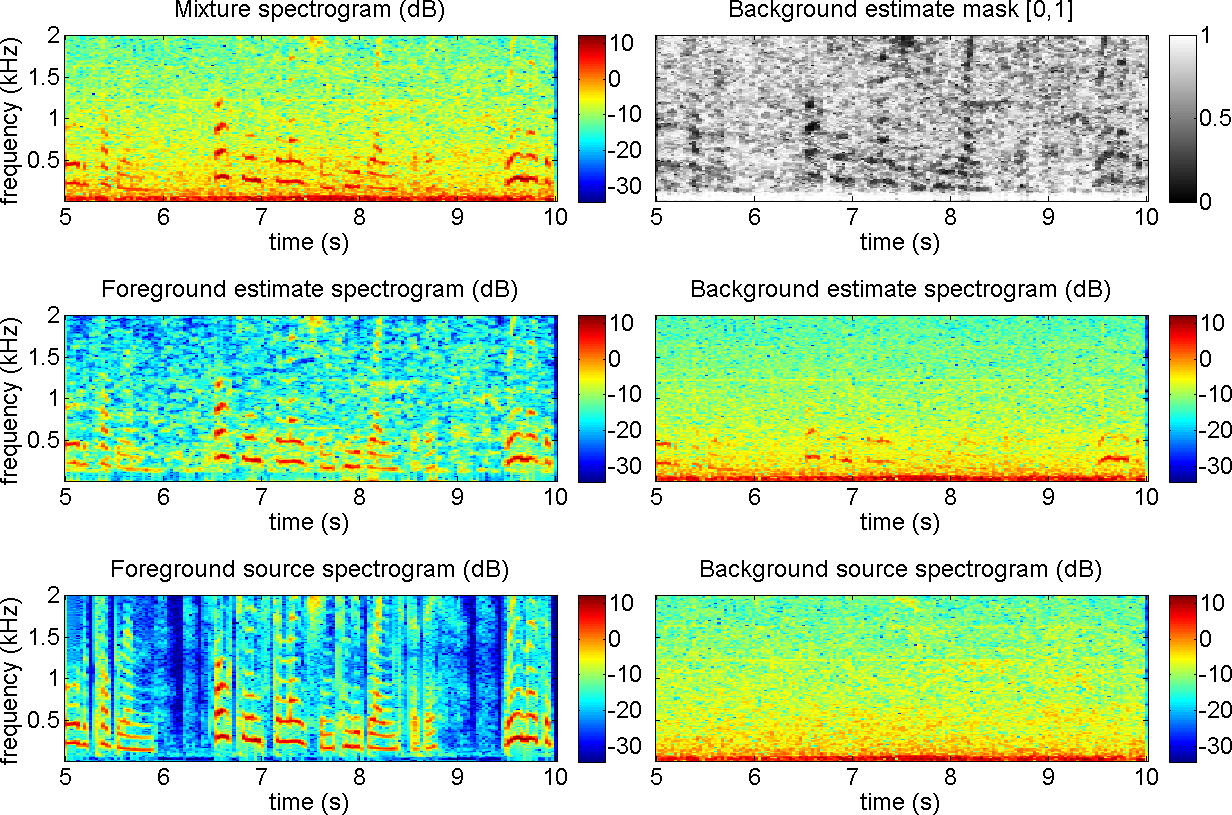
\includegraphics[width=\columnwidth]{Images/repet_sim_example.png}
\caption{Noise/speech separation using REPET-SIM. The mixture is a female speaker (foreground) speaking in a town square (background). The square has repeating noisy elements (passers-by and cars) that happen intermittently. The spectrograms and the mask are shown for 5 seconds and up to 2 kHz.}
\label{fig:repet_sim_example}
\end{figure}

\begin{itemize}[noitemsep,topsep=0pt]
\item \href{Audio/REPET/dev_Sq1_Co_B_mix.wav}{Mixture}
\item Estimates: \href{Audio/REPET/dev_Sq1_Co_B_mix_foreground.wav}{foreground} - \href{Audio/REPET/dev_Sq1_Co_B_mix_background.wav}{background}
\item Originals: \href{Audio/REPET/dev_Sq1_Co_B_sim.wav}{speech} - \href{Audio/REPET/dev_Sq1_Co_B_noi.wav}{noise}
\end{itemize}

For more information on this project, the reader is referred to \cite{inproceedings_rafii_oct2012}, \cite{inproceedings_rafii_may2013}, and \cite{inbook_rafii_2014}.


\subsection{uREPET (2015)}
\label{ssec:urepet}

Repetition is a fundamental element in generating and perceiving structure in audio. Especially in music, structures tend to be composed of patterns that repeat through time (e.g., rhythmic elements in a musical accompaniment), and also frequency (e.g., different notes of the same instrument). The auditory system has the remarkable ability to parse such patterns by identifying repetitions within the audio mixture. On this basis, we propose a simple user interface system for recovering patterns repeating in time and frequency in mixtures of sounds. A user selects a region in the log-frequency spectrogram of an audio recording from which she/he wishes to recover a repeating pattern covered by an undesired element (e.g., a note covered by a cough). The selected region is then cross-correlated with the spectrogram to identify similar regions where the underlying pattern repeats. The identified regions are finally averaged over their repetitions and the repeating pattern is recovered.

\begin{figure}[!htb]
\centering
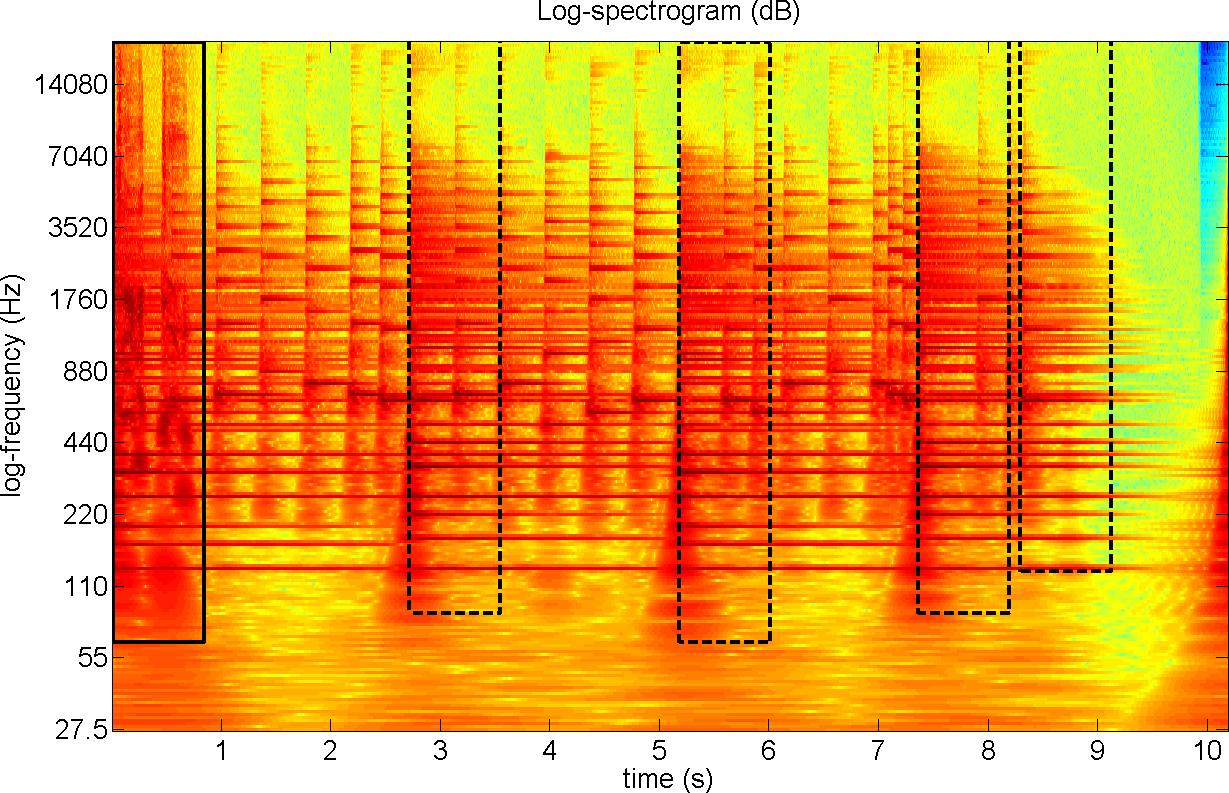
\includegraphics[width=\columnwidth]{Images/urepet_example1a.png}
\caption{Log-spectrogram of a melody with a cough covering the first note. The user selected the region of the cough (solid line) and the system identified similar regions where the underlying note repeats (dashed lines).}
\label{fig:urepet_example1a}
\end{figure}

\begin{figure}[!htb]
\centering
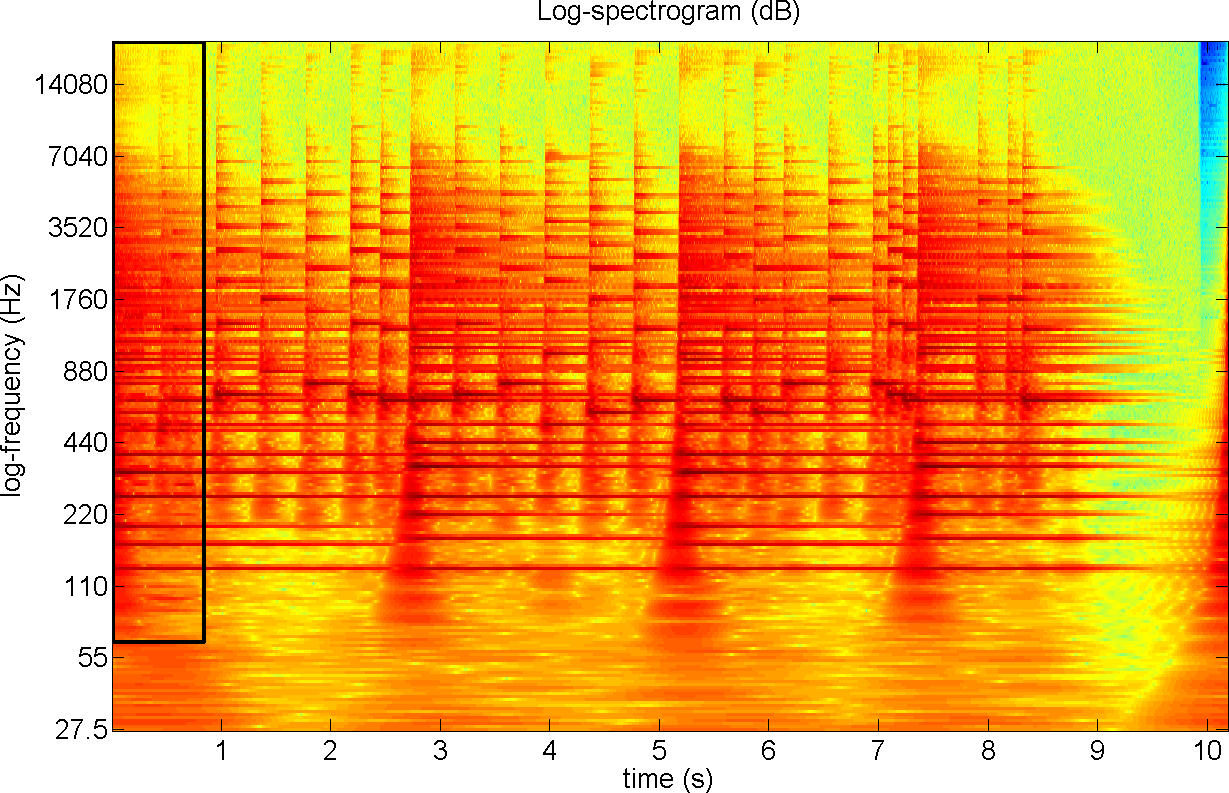
\includegraphics[width=\columnwidth]{Images/urepet_example1b.png}
\caption{Log-spectrogram of the melody with the first note recovered. The system averaged the identified regions over their repetitions and filtered out the cough from the selected region.}
\label{fig:urepet_example1b}
\end{figure}

\begin{itemize}[noitemsep,topsep=0pt]
\item \href{Audio/uREPET/melody&cough.wav}{Melody covered by a cough}
\item \href{Audio/uREPET/melody-cough.wav}{Recovered melody}
\item \href{Audio/uREPET/melody.wav}{Original melody} - \href{Audio/REPET/cough.wav}{original cough}
\end{itemize}

\begin{figure}[!htb]
\centering
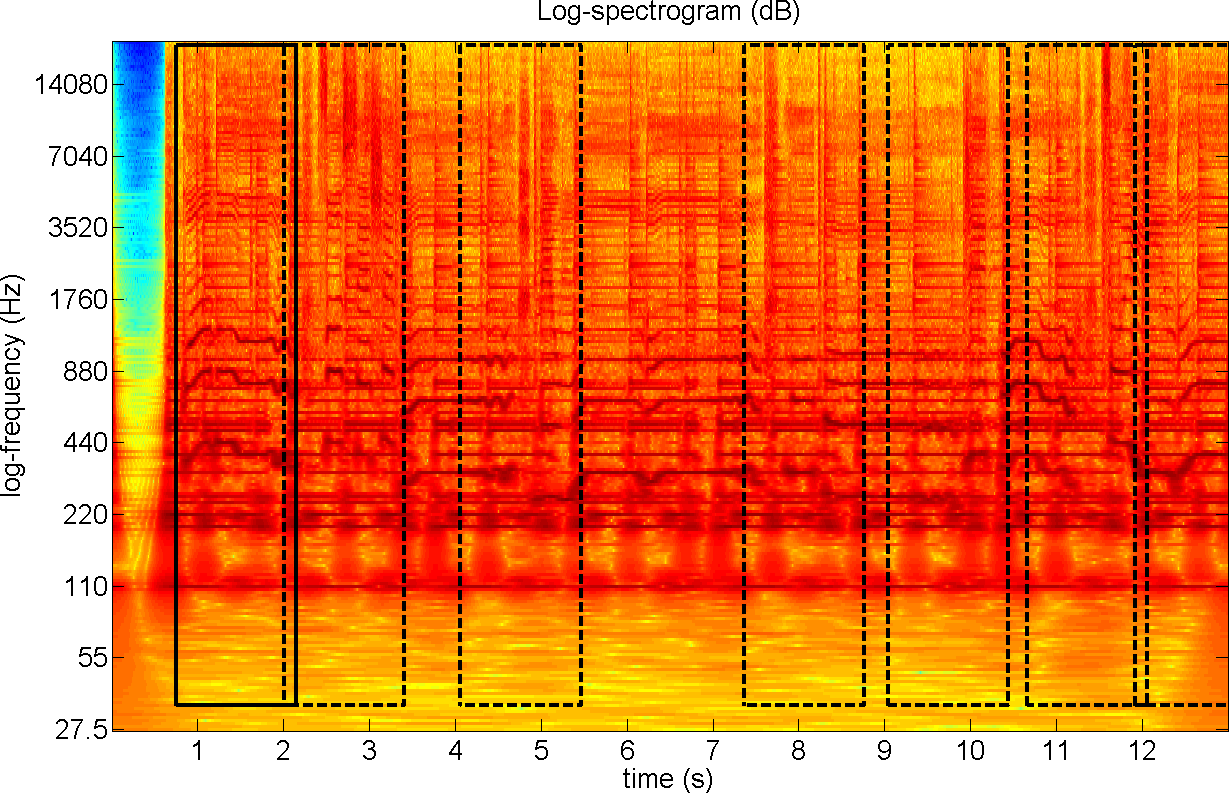
\includegraphics[width=\columnwidth]{Images/urepet_example2a.png}
\caption{Log-spectrogram of a song with vocals covering an accompaniment. The user selected the region of the first measure (solid line) and the system identified similar regions where the underlying accompaniment repeats (dashed lines).}
\label{fig:urepet_example2a}
\end{figure}

\begin{figure}[!htb]
\centering
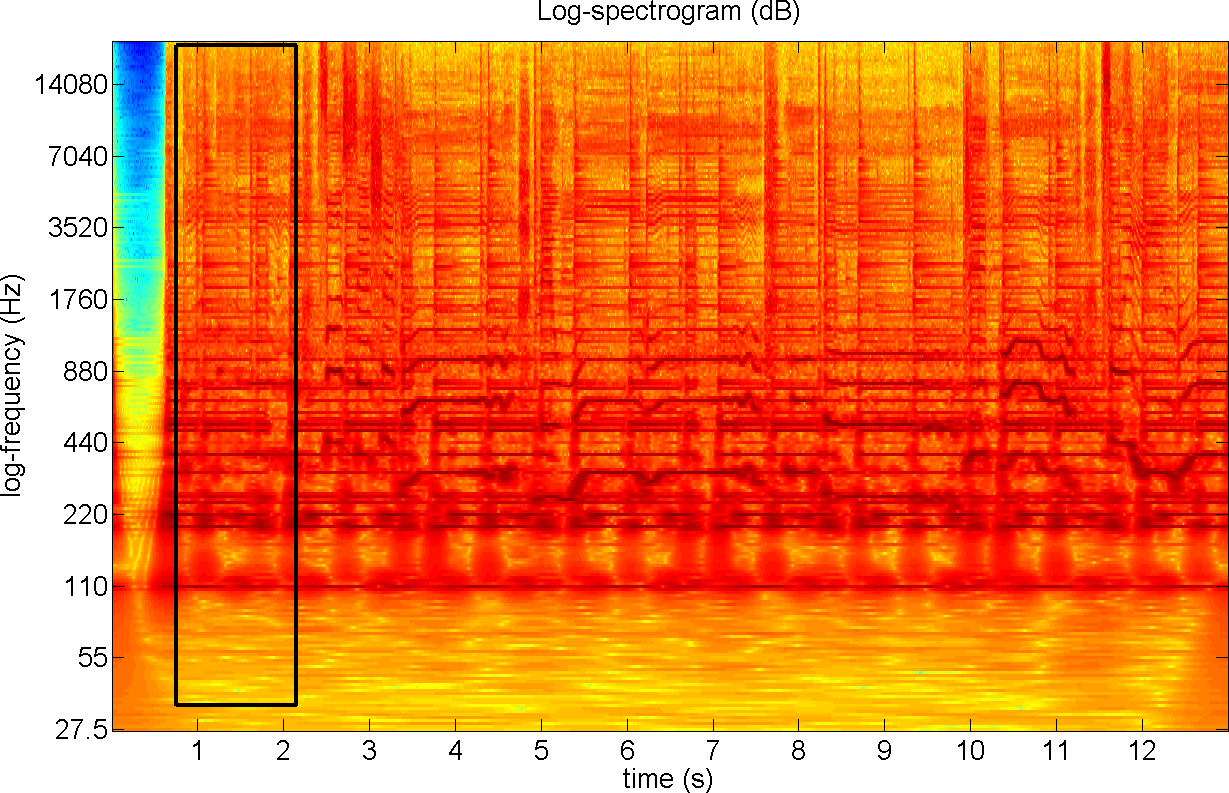
\includegraphics[width=\columnwidth]{Images/urepet_example2b.png}
\caption{Log-spectrogram of the song with the first measure of the accompaniment recovered. The system averaged the identified regions over their repetitions and filtered out the vocals from the selected region.}
\label{fig:urepet_example2b}
\end{figure}

\begin{itemize}[noitemsep,topsep=0pt]
\item \href{Audio/uREPET/accompaniment&vocals.wav}{Accompaniment covered by vocals}
\item \href{Audio/uREPET/accompaniment-vocals.wav}{Recovered accompaniment}
\item \href{Audio/uREPET/accompaniment.wav}{Original accompaniment} - \href{Audio/REPET/vocals.wav}{original vocals}
\end{itemize}

\begin{figure}[!htb]
\centering
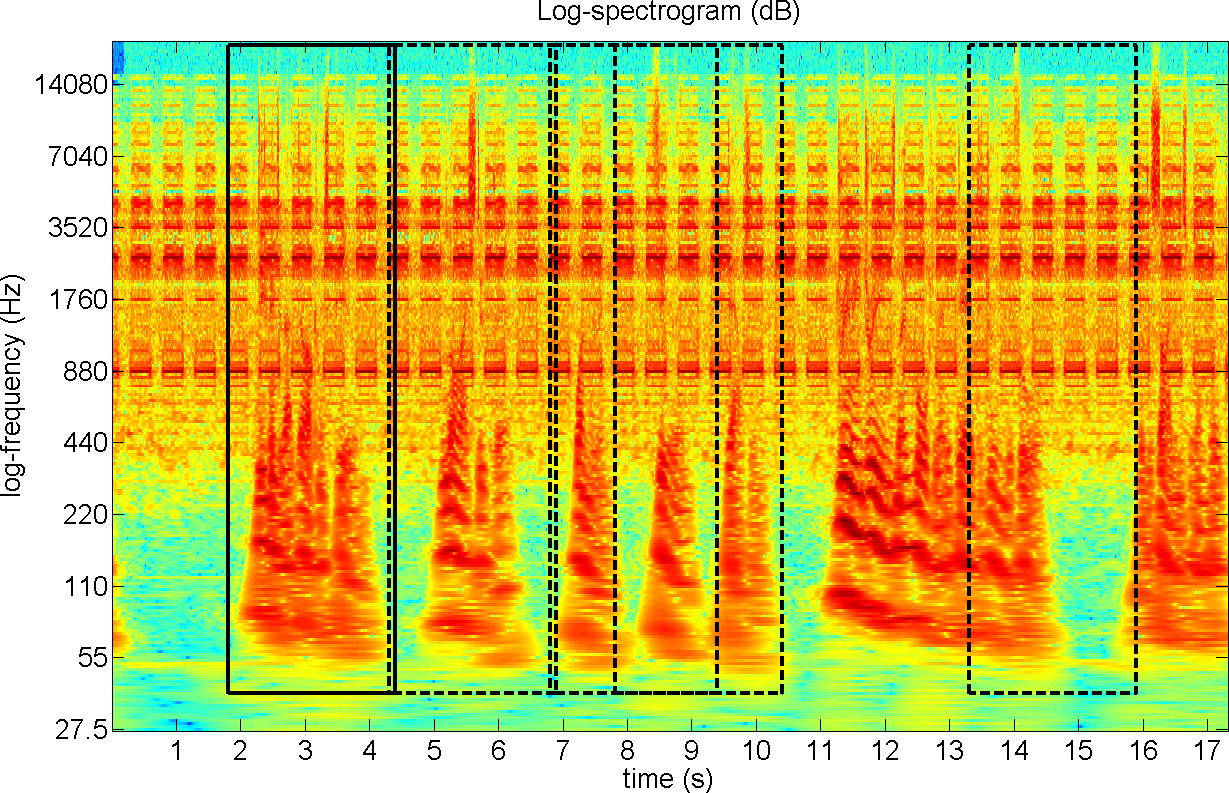
\includegraphics[width=\columnwidth]{Images/urepet_example3a.png}
\caption{Log-spectrogram of a speech covering a noise. The user selected the region of the first sentence (solid line) and the system identified similar regions where the underlying noise repeats (dashed lines).}
\label{fig:urepet_example3a}
\end{figure}

\begin{figure}[!htb]
\centering
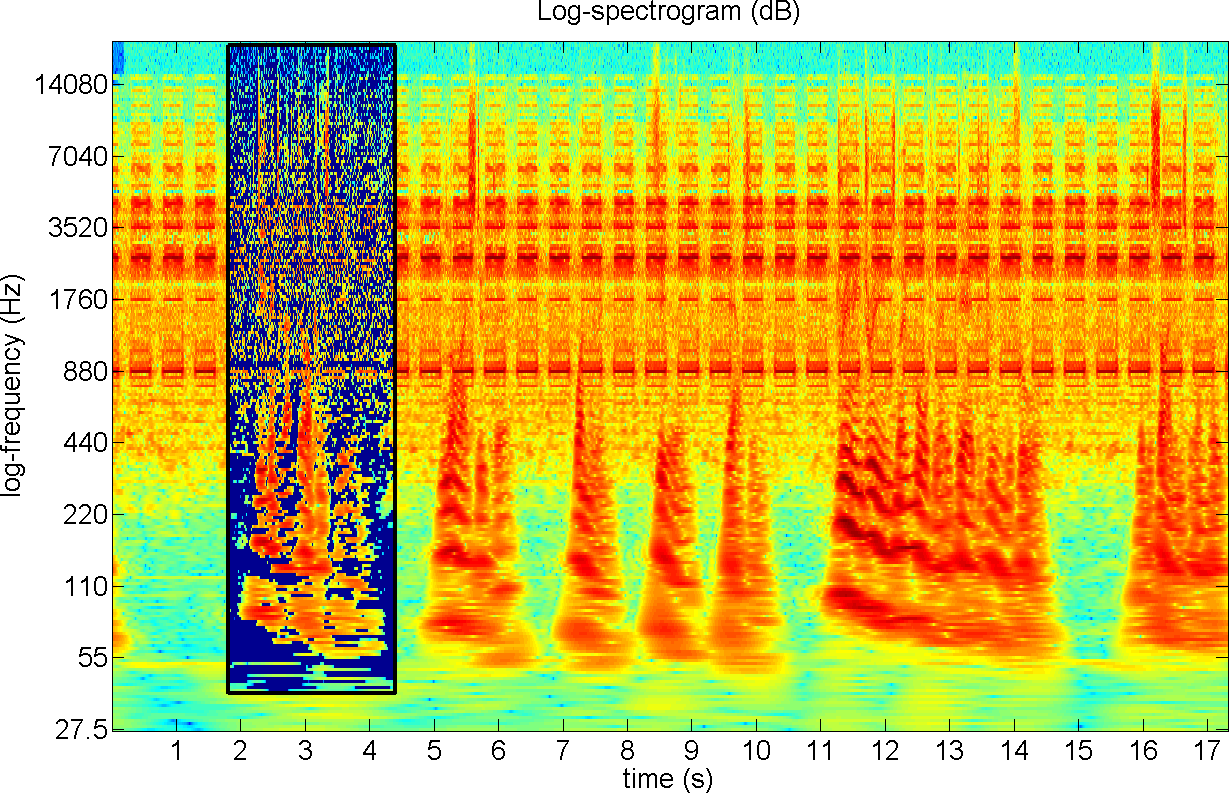
\includegraphics[width=\columnwidth]{Images/urepet_example3b.png}
\caption{Log-spectrogram of the first sentence of the speech extracted. The system averaged the identified regions over their repetitions and extracted the speech from the selected region.}
\label{fig:urepet_example3b}
\end{figure}

\begin{itemize}[noitemsep,topsep=0pt]
\item \href{Audio/uREPET/speech&noise.wav}{Speech covering a noise}
\item \href{Audio/uREPET/speech-noise.wav}{Recovered speech}
\item \href{Audio/uREPET/speech.wav}{Original speech} - \href{Audio/REPET/noise.wav}{original noise}
\end{itemize}

For more information on this project, the reader is referred to \cite{inproceedings_rafii_apr2015}.


\subsection{PROJET-MAG (2017)}
\label{ssec:projet-mag}

We propose a simple user-assisted method for the recovery of repeating patterns in time and frequency which can occur in mixtures of sounds. Here, the user selects a region in a logfrequency spectrogram from which they seek to recover the underlying pattern which is obscured by another interfering source, such as a chord masked by a cough. A cross-correlation is then performed between the selected region and the spectrogram, revealing similar regions. The most similar region is then selected and a variant on the PROJET algorithm, termed PROJET-MAG, is then used to extract the common time-frequency components from the two regions, as well as extracting the components which are not common to both. The results obtained are compared to another user-assisted method based on REPET, and the PROJET-MAG method is demonstrated to give improved results over this baseline.

\begin{itemize}[noitemsep,topsep=0pt]
\item \href{Audio/uREPET/melody&cough.wav}{Melody covered by a cough}
\item \href{Audio/uREPET/melody-cough (uREPET).wav}{Recovered melody uREPET} - \href{Audio/uREPET/melody-cough (PROJET-MAG).wav}{PROJET-MAG}
\item \href{Audio/uREPET/melody.wav}{Original melody} - \href{Audio/REPET/cough.wav}{original cough}
\end{itemize}

\begin{itemize}[noitemsep,topsep=0pt]
\item \href{Audio/uREPET/accompaniment&vocals.wav}{Accompaniment covered by vocals}
\item \href{Audio/uREPET/accompaniment-vocals (uREPET).wav}{Recovered accompaniment uREPET} - \href{Audio/uREPET/accompaniment-vocals (PROJET-MAG).wav}{PROJET-MAG}
\item \href{Audio/uREPET/accompaniment.wav}{Original accompaniment} - \href{Audio/REPET/vocals.wav}{original vocals}
\end{itemize}

\begin{itemize}[noitemsep,topsep=0pt]
\item \href{Audio/uREPET/speech&noise.wav}{Speech covering a noise}
\item \href{Audio/uREPET/speech-noise.wav (uREPET)}{Recovered speech uREPET} - \href{Audio/uREPET/speech-noise.wav (PROJET-MAG)}{PROJET-MAG}
\item \href{Audio/uREPET/speech.wav}{Original speech} - \href{Audio/REPET/noise.wav}{original noise}
\end{itemize}

For more information on this project, the reader is referred to \cite{inproceedings_fitzgerald_mar2017}.


\section{Codes}
\label{sec:codes}

\subsection{Zaf-Python}
\label{ssec:zaf-python}

This \href{https://github.com/zafarrafii/Zaf-Python}{GitHub repository} contains Zafar's Audio Functions in \textbf{Python} for audio signal analysis: STFT, inverse STFT, mel filterbank, mel spectrogram, MFCC, CQT kernel, CQT spectrogram, CQT chromagram, DCT, DST, MDCT, inverse MDCT.

\begin{figure}[!htb]
\centering
\begin{minipage}[b]{\columnwidth}
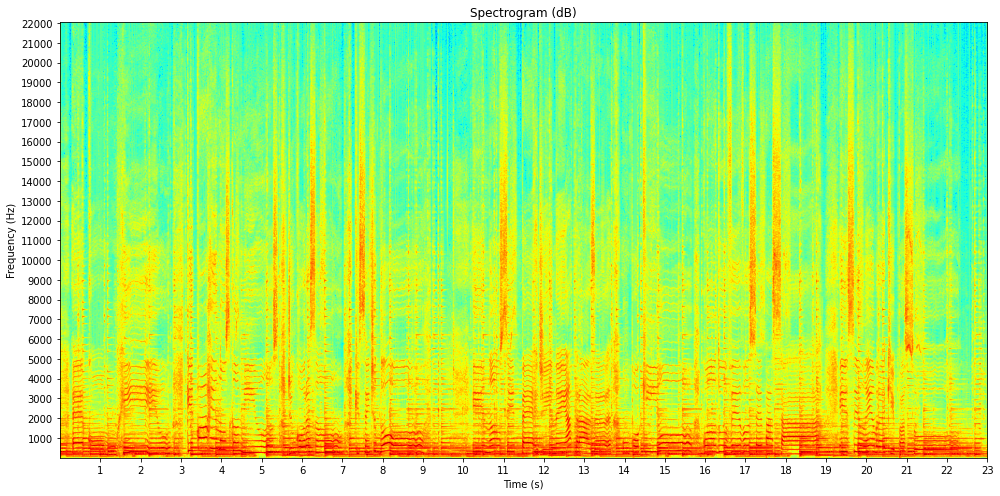
\includegraphics[width=\columnwidth]{Images/stft.png}
\end{minipage}
\begin{minipage}[b]{\columnwidth}
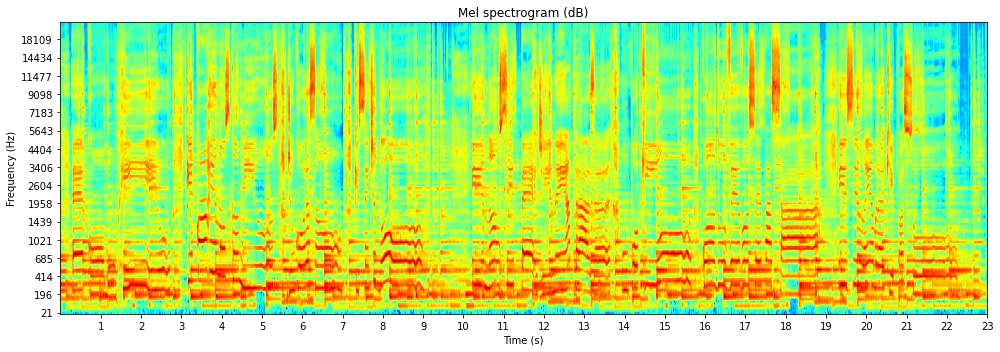
\includegraphics[width=\columnwidth]{Images/melspectrogram.png}
\end{minipage}
\begin{minipage}[b]{\columnwidth}
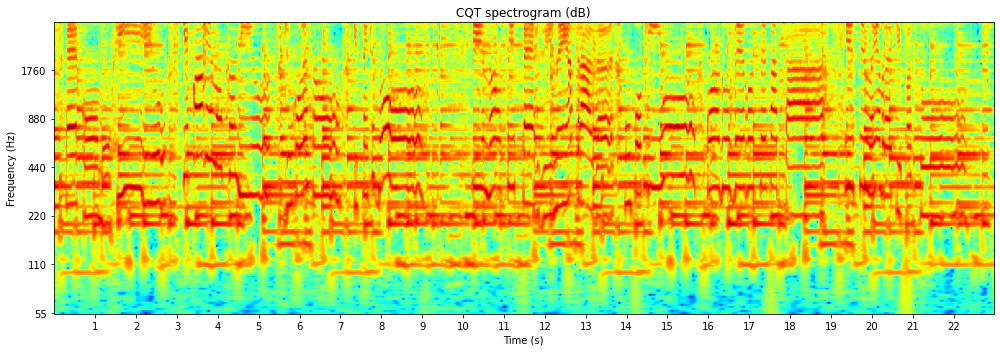
\includegraphics[width=\columnwidth]{Images/cqtspectrogram.png}
\end{minipage}
\caption{STFT spectrogram, mel spectrogram, and CQT spectrogram (from top to bottom) computed using the Zaf-Python module.}
\label{fig:zaf-python}
\end{figure}


\subsection{Zaf-Matlab}
\label{ssec:zaf-matlab}

This \href{https://github.com/zafarrafii/Zaf-Matlab}{GitHub repository} contains Zafar's Audio Functions in \textbf{Matlab} for audio signal analysis: STFT, inverse STFT, mel filterbank, mel spectrogram, MFCC, CQT kernel, CQT spectrogram, CQT chromagram, DCT, DST, MDCT, inverse MDCT. See also \href{https://www.mathworks.com/matlabcentral/fileexchange/90501-zaf-matlab}{MathWorks' File Exchange}.


\subsection{Zaf-Julia}
\label{ssec:zaf-julia}

This \href{https://github.com/zafarrafii/Zaf-Julia}{GitHub repository} contains Zafar's Audio Functions in \textbf{Julia} for audio signal analysis: STFT, inverse STFT, mel filterbank, mel spectrogram, MFCC, CQT kernel, CQT spectrogram, CQT chromagram, DCT, DST, MDCT, inverse MDCT.


\subsection{REPET-Python}
\label{ssec:repet-python}

This \href{https://github.com/zafarrafii/REPET-Python}{GitHub repository} contains REPET in \textbf{Python} for audio source separation: original REPET, REPET extended, adaptive REPET, REPET-SIM, and online REPET-SIM.

\begin{figure}[!htb]
\centering
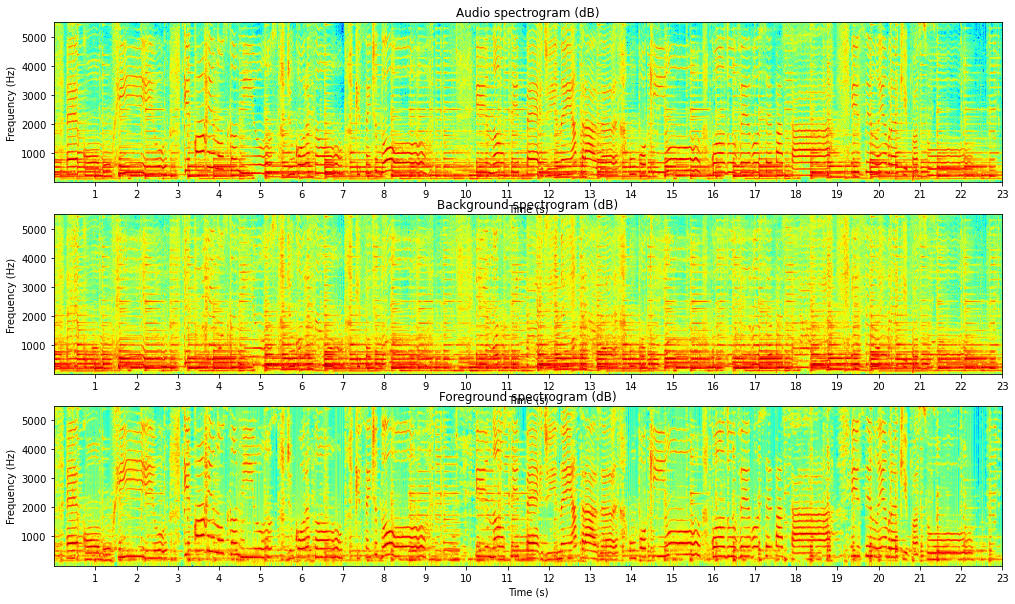
\includegraphics[width=\columnwidth]{Images/repet_original.png}
\caption{Separation of a musical excerpt into its accompaniment background and vocal foreground estimates (from top to bottom) using the original REPET from the REPET-Python module.}
\label{fig:repet_original}
\end{figure}


\subsection{REPET-Matlab}
\label{ssec:repet-matlab}

This \href{https://github.com/zafarrafii/REPET-Matlab}{GitHub repository} contains REPET in \textbf{Matlab} for audio source separation: original REPET, REPET extended, adaptive REPET, REPET-SIM, and online REPET-SIM. See also \href{https://www.mathworks.com/matlabcentral/fileexchange/88803-repet-matlab}{MathWorks' File Exchange}.


\subsection{REPET-GUI-Matlab}
\label{ssec:repet-gui-matlab}

This \href{https://github.com/zafarrafii/REPET-GUI-Matlab}{GitHub repository} contains Matlab GUIs to demo the original REPET and REPET-SIM. See also \href{https://www.mathworks.com/matlabcentral/fileexchange/90736-repet-gui-matlab}{MathWorks' File Exchange}.


\subsection{uREPET-Matlab}
\label{ssec:urepet-matlab}

This \href{https://github.com/zafarrafii/uREPET-Matlab}{GitHub repository} contains a Matlab GUI for uREPET, a simple user interface system for recovering patterns repeating in time and frequency in mixtures of sounds. See also \href{https://www.mathworks.com/matlabcentral/fileexchange/90606-urepet-matlab}{MathWorks' File Exchange}.


\subsection{Zap-Matlab}
\label{ssec:zap-matlab}

This \href{https://github.com/zafarrafii/Zap-Matlab}{GitHub repository} contains a Matlab GUI which implements Zafar's audio player (Zap), featuring some practical functionalities such as a playback line, a select/drag tool, and a synchronized spectrogram. See also \href{https://www.mathworks.com/matlabcentral/fileexchange/90741-zap-matlab}{MathWorks' File Exchange}.


\subsection{CQHC-Python}
\label{ssec:cqhc-python}

This \href{https://github.com/zafarrafii/CQHC-Python}{GitHub repository} contains a Python implementation for the CQHCs, including a module with the MFCCs, the CQT spectrogram, the CQT deconvolution, and the CQHCs themselves, and notebooks with examples, tests, and notes.


\subsection{Problems-Python}
\label{ssec:problems-python}

This \href{https://github.com/zafarrafii/Problems-Python}{GitHub repository} contains Jupyter notebooks with Python coding problems (and solutions). These can be good exercises for beginners and more experienced users to improve and review their programming skills in Python. 


\printbibheading[title={References},heading=bibnumbered]
\label{sec:refs}
\printbibliography[title={Patents},type=patent,heading=subbibnumbered]
\printbibliography[title={Journal Articles},type=article,heading=subbibnumbered]
\printbibliography[title={Conference Proceedings},type=inproceedings,heading=subbibnumbered]
\printbibliography[title={Book Chapters},type=inbook,heading=subbibnumbered]
\printbibliography[title={Technical Reports},type=report,heading=subbibnumbered]
\printbibliography[keyword={tutorial},title={Tutorials},type=misc,heading=subbibnumbered]
\printbibliography[keyword={workshop},title={Workshops},type=misc,heading=subbibnumbered]
\printbibliography[keyword={talk},title={Talks},type=misc,heading=subbibnumbered]
\printbibliography[keyword={lecture},title={Lectures},type=misc,heading=subbibnumbered]
\printbibliography[title={Data Sets},type=online,heading=subbibnumbered]

\end{document}
